\chapter{Lasso i lineære modeller}
\textit{I dette kapital introduceres lasso estimatoren for lineære modeller og generaliseringen af denne !!!}

Vi betragter et sædvanligt lineær regression set-up. Lad $\textbf{y} = \del{y_1, \dots, y_n}^T$ være respons variablen og lad $\textbf{X} = \del{\textbf{x}_1, \dots, \textbf{x}_n}$ være en $n \times p$ matrix af prædiktorer, hvor $\textbf{x}_j = \del{x_{1,j}, \dots, x_{n,j}}^T$, $j = 1, \dots, p$ er vektorer af prædiktorer. 
Vi antager en lineær funktion af prædiktorer, som har normal fordelte fejl. 
\begin{align*}
\textbf{y} = \textbf{X} \mathcal{\beta} + \epsilon, \quad \epsilon \sim N \del{0, \sigma^2 \text{\textbf{I}}_n},
\end{align*}
hvor $\mathcal{\beta} = \del{\beta_1, \dots, \beta_p}^T$ er en vektor af ukendte parameter og $\text{\textbf{I}}_n$ er $n \times n$ identitetsmatricen. 
For nu antager vi, at $p<n$ og at første kolonne i $\X$ er alle elementer 1'taller. 
Vi angiver $\widehat{\boldsymbol{\beta}}^{OLS}$ til at være den mindste kvadraters estimat;
\begin{align*}
\widehat{\boldsymbol{\beta}}^{OLS} = \underset{\boldsymbol\beta \in \R^p}{\argmin} \norm{ \textbf{y} - \textbf{X}\boldsymbol\beta}^2_2
\end{align*}
Den velkendte løsning er givet ved 
\begin{align*}
\widehat{\boldsymbol\beta}^{\text{OLS}} = \del{\X^T \X}^{-1} \X^T \y.
\end{align*}
For at inverterer $\X^T \X$ skal $\X$ have fuld rang ellers er $\widehat{\boldsymbol\beta}^{\text{OLS}}$ ikke unik. 
Men når  \(p \gg n\) vil prædiktorerne være kollineære og dermed har \(\X\) ikke fuld rang.
Det betyder, at $\X^T \X$ er singulær og der findes derfor en ikke entydig estimator for mindste kvadraters metode.
%En løsning til dette kan være at tilføje et positiv værdi til diagonalen af $\X^T \X$, som vil medfører en entydig løsning . 
%Estimatet vil derfor have formen
%\begin{align*}
% \del{\X^T \X + \lambda \text{\textbf{I}}_p}^{-1} \X^T \y,
%\end{align*}
%hvor $\lambda > 0$ og kaldes strafparameteren. Den overstående formel er løsning til \textit{ridge regression problemet}:
%\begin{align}
% \widehat{\boldsymbol\beta}^{\text{R}} = \underset{\boldsymbol\beta \in \R^p}{\argmin}  \cbr{\norm{\y - \X\beta}^2_2 + \lambda \norm{\boldsymbol\beta}_2^2},
%\end{align}
%som er beskrevet, som et lagrange problem. 
%Det kan også kan skrives til et betingede problem 
%\begin{align}
% \widehat{\boldsymbol\beta}^{\text{R}} = \underset{\boldsymbol{\beta} \in \R^p}{\argmin} \cbr{\norm{\y - \X\boldsymbol\beta}^2_2} \quad \text{underlagt at } \quad \norm{\boldsymbol\beta}_2^2 < t 
%\end{align}
%Der er en en-til-en korrespondance mellem det betingede problem \eqref{eq:2.7} og Lagrange problemet \eqref{eq:2.8}.
%Første led i \eqref{eq:2.8} svarer til OLS, som finder de estimerede koefficienter ved at minimere SSR, mens sidste led mindsker de estimerede koefficienter .



%Betragt \(n\) observationer \(\{x_i, y_i\}_{i=1}^n \), hvor $x_i=(x_{i1}, \ldots, x_{ip})$ er en $p$ dimensional vektor af forklarende variable eller prædiktorer og $y_i \in \R$ er den tilhørende respons variabel.
%
%Den velkendte estimator for mindste kvadraters metode for $(\beta_0, \beta)$ findes udfra
%\begin{align*}
%\min_{\beta_0, \beta} \cbr{\frac{1}{2n} \sum_{i=1}^n \del{y_i - \beta_0 - \sum_{j=1}^p x_{ij} \beta_j}^2}
%\end{align*}
%Løsningen hertil er givet ved
%\begin{align*}
%\hat{\beta}^{\text{OLS}} = (\X^T \X)^{-1} \X^T \y.
%\end{align*}

%Som bekendt er estimatoren unbiased, men ofte har den en høj varians.


%Hvis \(p \gg n\) da vil prediktorerne være kollineære og dermed har \(\X\) ikke fuld rang.
%Det betyder, at $\X^T \X$ er singulær og der findes derfor en ikke entydig estimator for mindste kvadraters metode.


Nedenfor introduceres lasso som kombinerer objektfunktionen for mindste kvadraters metode med en $\ell_1$ betingelse. Denne betingelse mindsker koefficienterne og sætter endda nogle lig 0. Dermed udfører lasso model udvælgelse.
\section{Lasso estimatoren} \label{sec:lasso_estimatoren}
\textit{Dette afsnit er skrevet udfra kapitel 2 i \citep{hastie}.}

\textit{The Least Absolute Shrinkage Selection Operator}, som forkortes lasso, blev introduceret af \citep{lasso}. 
Lasso finder løsningen til optimeringsproblemet
\begin{align}
\arg \min_{\beta} \cbr{\frac{1}{2n} \sum_{i=1}^n \del{y_i - \sum_{j=1}^p x_{ij} \beta_j}^2}, \ \text{underlagt at } \sum_{j=1}^p \vert \beta_j \vert \leq t, \label{eq:2.3}
\end{align} 
hvor vi bemærker, at betingelsen $\sum_{j=1}^p \vert \beta_j \vert \leq t$ kan skrives mere kompakt som en \(\ell_1\)-norm betingelse $\Vert \beta \Vert_1 \leq t$.

%På matrix-vektor form omskrives \eqref{eq:2.3} til
%\begin{align*}
%\arg \min_{ \beta} \cbr{\frac{1}{2n} \Vert \y - \X \beta \Vert_2^2}, \ \text{underlagt at } \Vert \beta \Vert_1 \leq t,
%\end{align*}
%hvor \(\Vert \cdot \Vert_2\) betegner den Euklidiske norm.
Værdi af \(t\) begrænser summen af de absolutte værdier af parameter estimaterne.
Den kontrollerer kompleksiteten af modellen. 
Større værdi af \(t\) betyder flere parametre og tillader dermed at modellen tilpasser data meget præcis.
Mindre værdi af \(t\) vil begrænse antallet af parametre, hvilket fører til mere sparse modeller, som tilpasser data mindre præcis.
Værdien af \(t\) skal specificeres ved en ekstern procedure kaldet \textit{krydsvalidering}, som vil blive diskuteret i kapitel \ref{kap:statistisk_inferens}.

Lasso problemet kan omskrives til Lagrange form
\begin{align}
\hat{\beta}^\text{lasso} = \arg \min_{\beta} \cbr{\frac{1}{2n} \Vert \y - \X \beta \Vert_2^2 + \lambda \Vert \beta \Vert_1}, \label{eq:2.5}
\end{align}
hvor $\lambda \geq 0$ er en såkaldt strafparameter, som også bestemmes udfra krydsvalidering. 
Der er en en-til-en korrespondance mellem det betingede problem \eqref{eq:2.3} og Lagrange problemet \eqref{eq:2.5}. 
For hver værdi af \(t\) hvor \(\Vert \beta \Vert_1 \leq t\) er opfyldt, da findes en tilhørende værdi af $\lambda$ som giver den samme løsning for \eqref{eq:2.5}.
Omvendt gælder der, at løsningen $\hat{\beta}_\lambda$ til \eqref{eq:2.5} løser grænse problemet med $t=\Vert \hat{\beta}_\lambda \Vert_1$.

I andre beskrivelser af lasso estimatoren ses det at faktoren \(\frac{1}{2n}\) i \eqref{eq:2.3} og \eqref{eq:2.5} erstattes med \(\frac{1}{2}\) eller \(1\).
Dette gør ingen forskel i \eqref{eq:2.3} og svarer blot til en simpel reparametrisering af \(\lambda\) i \eqref{eq:2.5}.
Denne standardisering gør \(\lambda\) værdierne sammenlignelige for samples size af forskellige størrelse, som er brugbart i krydsvalidering.

\textit{Ridge regression} estimatoren findes udfra 
\begin{align} 
\hat{\beta}^\text{ridge} = \arg \min_{\beta} \cbr{\frac{1}{2n} \sum_{i=1}^n \del{y_i - \sum_{j=1}^p x_{ij} \beta_j}^2}, \ \text{underlagt at } \sum_{j=1}^p \beta_j^2 \leq t, \label{eq:2.7} 
\end{align} 
%som kan omskrives på Lagrange form
%\begin{align} 
%\arg \min_{\beta} \cbr{\frac{1}{2n} \sum_{i=1}^n \del{y_i - \sum_{j=1}^p x_{ij} \beta_j}^2 + \lambda \sum_{j=1}^p \beta_j^2}, 
%\end{align} \label{eq:2.8} 
%hvor $\lambda \geq 0$.
som kan omskrives på Lagrange form
\begin{align*}
\hat{\beta}^\text{ridge} = \arg \min_{\beta} \cbr{\frac{1}{2n} \Vert \y - \X \beta \Vert_2^2 + \lambda \Vert \beta \Vert_2^2},
\end{align*}
hvor $\lambda \geq 0$.
Heraf kan ridge regression estimatoren findes ved at differentiere \(\del{\y - \X \beta}^T \del{\y - \X \beta} + \lambda \beta^T \beta\) mht $\beta$, sætte dette lig 0 og isolere for $\beta$. Hvoraf vi finder, at
\begin{align*} 
\hat{\beta}^\text{ridge} = (\X^T \X + \lambda I_p)^{-1} \X^T \y. 
\end{align*}  
I forhold til mindste kvadraters regression tilføjer ridge regression en positiv konstant $\lambda$ på diagonalen af $\X^T \X$, hvilket medfører, at \(\X^T \X\) er invertibel, selvom $\X$ ikke har fuld rang. 
Dermed er en entydig løsning altid garanteret. 

Lad os betragte data givet i tabel \ref{tab:crime}.
For 50 byer i United States er kriminalitetsraten per 1 million indbyggere givet og følgende 5 prædiktorer: 
\begin{itemize}
\item \texttt{funding}: årlige politiske finansiering i dollars per indbygger
\item \texttt{hs}: procentvise andel af 25 årige eller derover med 4 års gymnasial uddannelse
\item \texttt{not-hs}: procentvise andel af 16-19 årige som ikke går i gymnasiet og ikke har en gymnasiel uddannelse
\item \texttt{college}: procentvise andel af 18-24 årige som studerer på universitetet
\item \texttt{college4}: procentvise andel af 25 årige eller derover med mindst 4 år på universitetet
\end{itemize}
%
\begin{table}[ht] 
\centering 
\begin{tabular}{c|cccccc} 
\texttt{city} & \texttt{funding} & \texttt{hs} & \texttt{not-hs} & \texttt{college} & \texttt{college4} & \texttt{crime rate} \\
\midrule
1 & 40 & 74 & 11 & 31 & 20 & 478 \\
2 & 32 & 72 & 11 & 43 & 18 & 494 \\
3 & 57 & 70 & 18 & 16 & 16 & 643 \\
4 & 31 & 71 & 11 & 25 & 19 & 341 \\
5 & 67 & 72 & 9 & 29 & 24 & 773 \\
\vdots & \vdots & \vdots & \vdots & \vdots & \vdots & \vdots \\
50 & 66 & 67 & 26 & 18 & 16 & 940 \\
\bottomrule
\end{tabular}  
\caption{Kriminalitetsraten og fem prediktorer for \(n=50\) stater i United States.} \label{tab:crime} 
\end{table} 
%
Datasættet, som vi betegner crime data, er inkluderet for at underbygge teorien og vi vil løbende i rapporten referere til det.
På figur \ref{fig:crime_koef} anvendes crime data til at illustrere koefficientstierne for henholdsvis ridge regression og lasso.
%
\begin{figure}[H]
\centering
\begin{minipage}{0.4\linewidth}
\scalebox{0.32}{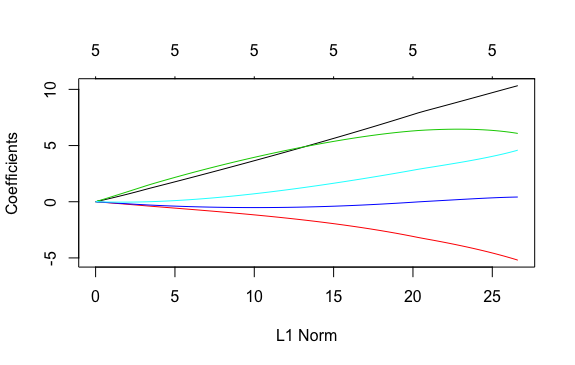
\includegraphics{fig/crime_ridge.png}}
\end{minipage}
\hspace{0.2cm}
\begin{minipage}{0.4\linewidth}
\scalebox{0.32}{\includegraphics{fig/crime_lasso.png}}
\end{minipage}
\caption{Koefficientstierne for ridge regression (venstre) og lasso (højre) plottet imod \(\ell_1\)-normen.} \label{fig:crime_koef}
\end{figure}

Variabel udvægelsen for ridge regression og lasso illustreres på figur \ref{fig:LassoRig}.
\begin{figure}[H]
\centering
\begin{minipage}{0.4\linewidth}
\scalebox{0.7}{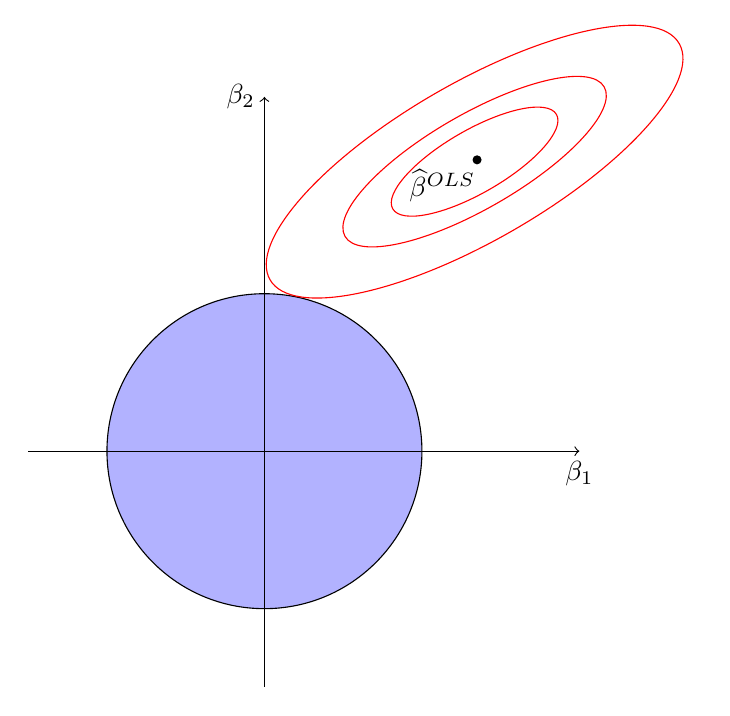
\begin{tikzpicture}
\draw [fill] (2.7,3.7) circle [radius=0.05];
\node [below left] (a) at (2.8,3.7) {$\widehat{\boldsymbol{\beta}}^\text{OLS}$};
\draw (0,0) circle (2cm) [fill= blue!30];
\draw [<-] (0,4.5) node [left] {$\beta_2$}-- (0,-3);
\draw[<-] (4,0) node [below] {$\beta_1$} -- (-3,0);
\begin{scope}[rotate = 30, red]
\clip[draw] (4.15,1.85) ellipse (3cm and 1cm);
\clip[draw] (4.15,1.85)ellipse (1.9 cm and 0.6 cm); 
\clip[draw] (4.15,1.85) ellipse (1.2 cm and 0.4 cm);
\end{scope}
\end{tikzpicture}}
\end{minipage}
\hspace{0.2cm}
\begin{minipage}{0.4\linewidth}
\scalebox{0.7}{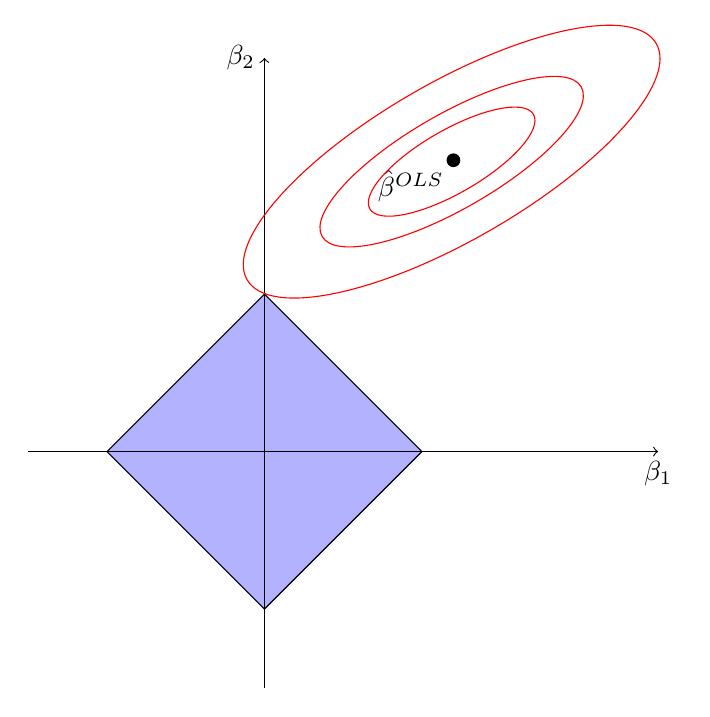
\begin{tikzpicture}
\draw [fill] (2.4,3.7) circle [radius=0.08];
\node [below left] (a) at (2.4,3.7) {$\hat{\beta}^\text{OLS}$};
\draw (-2,0) -- (0,2) -- (2,0)-- (0,-2) -- (-2,0)[fill = blue!30];
\draw [<-] (0,5) node [left] {$\beta_2$}-- (0,-3);
\draw[<-] (5,0) node [below] {$\beta_1$} -- (-3,0);
\begin{scope}[rotate = 30, red]
\clip[draw] (3.9,2) ellipse (3cm and 1cm);
\clip[draw] (3.9,2)ellipse (1.9 cm and 0.6 cm); 
\clip[draw] (3.9,2) ellipse (1.2 cm and 0.4 cm);
\end{scope}
\end{tikzpicture}}
\end{minipage}
\caption{Konturer for SSR og betingelsesområderne for ridge regression (venstre) og lasso (højre). De blå arealer er betingelsesområderne $\vert \beta_1 \vert+\vert \beta_2 \vert \leq t$ og $\beta_1^2+\beta_2^2 \leq t^2$, mens de røde ellipser er konturkurver for SSR. Konturkurverne har centrum i OLS estimatoren, $\hat{\beta}^\text{OLS}$.} \label{fig:LassoRig}
\end{figure}
For $p=2$ underligges OLS betingelsen $\beta_1^2 + \beta_2^2 \leq t^2$ for ridge regression og betingelsen $\vert \beta_1 \vert + \vert \beta_2 \vert \leq t$ for lasso.
Ellipserne omkring $\hat{\beta}^{\text{OLS}}$ er konturkurverne for SSR, dvs. SSR er konstant i en given ellipse. Værdien af SSR stiger, som ellipsen udvides fra $\hat{\beta}^{\text{OLS}}$.
Løsningen for ridge regression og lasso er givet ved det første punkt, hvor konturkurverne rammer betingelsesområderne.
Da ridge regression har et cirkulært betingelsesområde, vil skæringen med konturkurverne generelt ikke forekomme direkte på en akse.
Omvendt har lasso et regulært betingelsesområde med hjørner i hver akse, hvilket betyder, at hvis løsningen forekommer i et hjørne, da vil en af parametrene $\beta_j$ være lig 0.

Hvis $t$ er tilstrækkelig stor, da vil betingelsesområderne indeholde $\hat{\beta}^{\text{OLS}}$ og derfor vil ridge regression og lasso estimatorerne være lig OLS estimatoren.

På figur \ref{fig:LassoRig} har vi blot betragtet det simple tilfælde hvor $p=2$. Når $p=3$ vil betingelsesområdet for ridge regression være en kugle, mens betingelsesområdet for lasso vil være en polydron. 

\begin{lem}
Givet data \(\del{\y, \X}\), defineres et augmented datasæt
\begin{align*}
\mathbf{X}^* = \begin{bmatrix}
\mathbf{X} \\ \sqrt{\lambda} I_p
\end{bmatrix}, \quad 
\mathbf{y}^* = \begin{bmatrix}
\mathbf{y} \\ 0_p
\end{bmatrix},
\end{align*}
hvor \(\X^* \in \mathbb{R}^{\del{n+p} \times p}\) og \(\y^* \in \mathbb{R}^{n+p}\). Da kan estimatoren for ridge regression udledes udfra mindste kvadraters metode.
\end{lem}
\begin{proof}
Vi har, at
\begin{align*}
\del{\X^{*^T} \X^*}^{-1} \X^{*^T} \y^* &= \left( \begin{bmatrix}
\mathbf{X} & \sqrt{\lambda} I_p
\end{bmatrix}
\begin{bmatrix}
\mathbf{X} \\ \sqrt{\lambda} I_p
\end{bmatrix} \right)^{-1}
\begin{bmatrix}
\mathbf{X} & \sqrt{\lambda} I_p
\end{bmatrix}
\begin{bmatrix}
\mathbf{y} \\ 0
\end{bmatrix} \\
&= \left( \mathbf{X}^T \mathbf{X} + \lambda I_p \right)^{-1} \mathbf{X}^T \mathbf{y}.
\end{align*}
\end{proof}


\subsection{Udregning af lasso}
Da lasso strafleddet ikke er differentialbel, findes der ikke en eksplicit løsning til optimeringsproblemet for lasso.
En simpel procedure kaldet \textit{coordinate descent} kan udfra lagrange formen udregne en numerisk løsning. 

\subsubsection{Single prædiktor: soft tresholding}
Vi betragter blot en enkelt prædiktor \(z_i\). 
Problemet, som vi skal løse, er da
\begin{align*}
\arg \min_{\beta} \cbr{\frac{1}{2n} \sum_{i=1}^n \del{y_i - z_{i} \beta}^2 + \lambda \vert \beta \vert}.
\end{align*}
Som bekendt er standard proceduren at finde den første ordens afledede mht $\beta$, sætte denne lig 0 og isolere for $\beta$. 
Men vi bemærker, at \(\vert \beta \vert \) ikke har en afledt i $\beta=0$.
Vi kan dog fortsætte ...
Vi finder, at
\begin{align*}
\frac{\partial}{\partial \beta} \del{\frac{1}{2n} \sum_{i=1}^n \del{y_i - z_{i} \beta}^2 + \lambda \vert \beta \vert}
&= -\frac{1}{n} \sum_{i=1}^n \del{y_i - z_{i} \beta} z_i + \begin{cases}
-\lambda \quad &\beta < 0 \\
[-\lambda, \lambda] & \beta = 0 \\
\lambda & \beta >0 
\end{cases}  \\
&= -\frac{1}{n} \left\langle \mathbf{z}, \mathbf{y} \right\rangle + \beta + \begin{cases}
-\lambda \quad &\beta < 0 \\
[-\lambda, \lambda] & \beta = 0 \\
\lambda & \beta >0 
\end{cases},
\end{align*}
da $\frac{1}{n} \sum_{i=1}^n z_i^2=1$. Dette sættes lig 0 og vi isolerer $\beta$, hvoraf vi finder, at
\begin{align}
\hat{\beta} = \begin{cases}
\frac{1}{n} \left\langle \mathbf{z}, \mathbf{y} \right\rangle - \lambda, \quad &\frac{1}{n} \left\langle \mathbf{z}, \mathbf{y} \right\rangle > \lambda, \\
0 &\frac{1}{n} \left\langle \mathbf{z}, \mathbf{y} \right\rangle \leq \lambda, \\
\frac{1}{n} \left\langle \mathbf{z}, \mathbf{y} \right\rangle + \lambda, &\frac{1}{n} \left\langle \mathbf{z}, \mathbf{y} \right\rangle < \lambda.
\end{cases} \label{eq:2.10}
\end{align}
Definer \textit{soft-threshold operatoren}
\begin{align*}
S_\lambda\del{x}=\text{sign}\del{x} \del{\vert x \vert - \lambda}_+,
\end{align*}
som trækker argumentet $x$ mod 0 med $\lambda$, og sætter den lig med 0 hvis $\vert x \vert \leq \lambda$. 
Figur \ref{fig:soft_thresholding_fct} illustrerer operatoren.
Da kan vi omskrive \eqref{eq:2.10} til
\begin{align*}
\hat{\beta} = S_\lambda \del{\frac{1}{n} \left\langle \mathbf{z}, \mathbf{y} \right\rangle}.
\end{align*}
%
\begin{figure}[H]
\centering
\scalebox{0.8}{\begin{tikzpicture}
\draw (-2.5,-2.5) -- (2.5,2.5);
\draw[dashed] (-2.5,-1.7) -- (-0.75,0) -- (0.75,0) -- (2.5,1.7); 
\draw[dotted] (2.5,1.7) -- (2.5,2.5);
%\draw node [label={[xshift=0.5cm, yshift=-0.8cm]$\del{0,0}$}] {};
\draw node [label={[xshift=2.75cm, yshift=1.8cm]$\lambda$}] {};
\draw [<-] (0,3) node [left] {$S_\lambda \del{x}$}-- (0,-3);
\draw[<-] (3,0) node [below] {$x$} -- (-3,0);
\end{tikzpicture}}
\caption[optional short text]{Soft thresholding funktionen $S_\lambda\del{x}=\text{sign}\del{x} \del{\vert x \vert - \lambda}_+$.} \label{fig:soft_thresholding_fct}
\end{figure}
%
\subsubsection{Multiple prædiktorer: cyclic coordinate descent}
Herefter kan vi betragte multivariate prædiktorer. 
%Gentagne cycle gennem prædiktorerne i en fast, men vilkårlig orden $j=1, 2, \ldots, p$, hvor koefficienten $\beta_j$ opdateres i det $j$'te step, ved at minimere objektfunktionen i dens koordinat, mens de resterende koefficienter $\cbr{\hat{\beta}_k, k \neq j}$ fastholdes deres nuværende værdier. 
Vi kan opskrive objektfunktionen i \eqref{eq:2.5} som
\begin{align*}
\frac{1}{2n} \sum_{i=1}^n \del{y_i - \sum_{k \neq j} x_{ik} \beta_k - x_{ij} \beta_j}^2 + \lambda \sum_{j = 1}^p \vert \beta_j \vert
\end{align*}
Definer den partialle residual $r_i^{(j)}=y_i - \sum_{k \neq j} x_{ik} \hat{\beta}_k$, som fjerner nuværende fit fra den $j$'te prædiktor.
Da er den j'te koefficient opdateret ved
\begin{align}
\hat{\beta}_j = S_\lambda \del{\frac{1}{n} \left\langle \mathbf{x}_j, \mathbf{r}^{(j)} \right\rangle}, \label{eq:2.14}
\end{align}
hvor \(r_i = y_i - \sum_{j = 1}^p x_{ij} \hat{\beta}_j \) er de fulde residualer.
Den beskrevne algoritme svarer til metoden \textit{cyclical coordinate descent}, som minimerer en konveks objektfunktion langs hver koordinat af gangen.
Under milde regularitetsbetingelser konvergerer løsningen til et global optimum.
Fra opdateringen \eqref{eq:2.14} ser vi, at algoritmen foretager en univariat regression af den partial residual på hver prædiktor, cycling gennem prædiktorerne indtil konvergens. \\

Ofte er vi interesseret i, at finde lasso løsningen for en mængde af \(\lambda\) værdier og ikke blot én fast lambda.
\textit{pathwise coordinate descent} kan anvendes hertil, ved at begynde med en værdi af \(\lambda\) som præcis er høj nok således at den optimale løsning er vektor bestående af \(0\).
Denne værdi er lig \(\lambda_{\max}=\max_j \vert \frac{1}{2} \left\langle \mathbf{x}_j, \y \right\rangle \vert\).
Da kan vi aftage \(\lambda\) med en lille mængde og køre coordinate descent undtil konvergens.
Aftage \(\lambda\) igen og anvende den tidligere løsning som en warm start, da kan vi kører coordinate descent indtil konvergens.
Hermed kan vi udregne løsningen over en grid af \(\lambda\) værdier. \\

Coordinate descent er særlig hurtig til at løse lasso problemet, da koordinatvis minimering er tilgængelig \eqref{eq:2.14}, og dermed er en iterativ søgning langs hver koordinat ikke nødvendig.
Derudover udnytter coordinat descent at lasso giver sparse løsninger.
For tilstrækkelige høje \(\lambda\) værdier er de fleste koefficienter lig $0$. \\[2mm] 
%
\textit{Homotopy metoder} er en alternativ teknisk til at løse lasso problemet. Disse producerer en helt sti af løsninger i en frekventiel sekvens, ved at starte med nul.
Denne sti er faktisk piecewise lineær.
Algoritmen kaldet \textit{least angle regression} (LARS) er en homotopy metode som effektivt konstruerer piecewise lineære stier.
En mere teoretisk gennemgang af coordinate descent og LARS algoritmen er givet i kapitel \ref{kap:optimeringsmetoder}. \\[2mm]


Hvis prædiktorerne er ortogonale, dvs $\frac{1}{n} \left\langle \mathbf{x}_j, \mathbf{x}_k \right\rangle = 0$ for alle $j \neq k$.
Da reduceres opdateringen \eqref{eq:2.14} til
\begin{align*}
\hat{\beta}_j = S_\lambda \del{\frac{1}{n} \left\langle \mathbf{x}_j, \mathbf{y} \right\rangle},
\end{align*}
dermed er $\hat{\beta}_j$ blot soft-thresholded version af det univariate mindste kvadraters estimat af $\mathbf{y}$ regresseret imod $\mathbf{x}_j$. Således har vi en lukket løsning og ingen iterationer er påkrævet.

\subsection{Frihedsgrader}
Antag at, vi har \(p\) prediktorer og tilpasser en lineær regressions model udfra \(k\) af disse prediktorer.
Hvis disse \(k\) prediktorer vælges uafhængigt af responsvariablen, da "anvender" fitting proceduren \(k\) frihedsgrader.
Dvs at teststørrelsen for at teste hypotesen om at alle \(k\) koefficienter er 0, har en Chi-squared fordeling med \(k\) frihedsgrader.

Hvis valget af de \(k\) prediktorer afhænger af responsvariablen, da forventes det at fitting proceduren anvender mere end \(k\) frihedsgrader. 
Vi kalder sådan en fitting procedure \textit{adaptiv}, og tydeligvis er lasso et eksempel på dette.

Ligeledes er forward-stepwise proceduren adaptiv, hvor vi sekventiel tilføjer prediktorer som mindsker fejlen mest.
Her forventes det at modellen anvender mere end \(k\) frihedsgrader efter \(k\) step.
Derfor er antallet af frihedsgrader ikke nødvendigvis lig med antallet af ikke-nul koefficienter.

Men for lasso er antallet af frihedsgrader faktisk lig antallet af ikke-nul koefficienter, som vi nu vil beskrive.

Først defineres hvad vi mener med frihedsgrader for en adaptiv fitted model. 
Antag at, vi har en additive-error model
\begin{align*}
y_i = f \del{x_i} + \epsilon_i, \quad i = 1, \ldots, n,
\end{align*}
hvor \(f\) er ukendt og \(\epsilon_i \sim iid \del{0, \sigma^2}\).
Lad \(\hat{\y}\) betegne \(n\) sample prediktorer, da defineres 
\begin{align*}
\text{df}\del{\hat{\y}} := \frac{1}{\sigma^2} \sum_{i=1}^n \text{Cov}\del{\hat{y}_i, y_i}.
\end{align*}
Antal frihedsgrader svarer da til indflydelsen hver respons mål har på dens prediktion.
Desto bedre modellen tilpasser data, desto højere antal frihedsgrader.
Det kan vises at, lasso med en fast strafparameter \(\lambda\) er antallet af ikke-nul koefficienter \(k_\lambda\) et unbiased estimat af frihedsgrader.

Som nævnt ovenfor anvender forward-stepwise regression mere end \(k\) frihedsgrader efter \(k\) step.
Lasso udvælger ikke blot prediktorer, som bekendt øger antallet af frihedsgrader, men shrinks også koefficienterne mod 0 relativ til mindste kvadraters estimaterne.
Denne skrinkage er netop tilstrækkelig til at brige antallet af frihedsgrader til \(k\).
Dette resultat er særligt nyttig, da det giver et kvalitativ mål af mængden af fitting som vi har opnået ved ethvert punkt på lasso stien.
Generelt er bevises for dette resultat meget besværligt.
Men i det ortogonale tilfælde ...

Ideen tages et skridt videre i sektion \ref{subsec:kovarians_test} hvor vi beskriver \textit{kovarians testen} til at teste significancen af prediktorerne ift lasso.


\subsubsection{Ikke-negative garrote}
\textit{Ikke-negative garrote}, introduceret af \citep{nonnegative_garrote}, er en two-stage procedure. 
Givet et initial estimat af regression koefficienterne \(\tilde{\beta} \in \mathbb{R}^p\), kan vi løse optimeringsproblemet
\begin{align}
\hat{\beta}_j^\text{garotte} = \arg \min_{c \in \mathbb{R}^p}  \cbr{ \sum_{i=1}^n \del{y_i - \sum_{j=1}^p c_j x_{ij} \tilde{\beta}_j}^2}, \ \text{underlagt at } c_j \geq 0 \text{ og } \Vert c \Vert_1 \leq t. \label{eq:2.19}
\end{align}
Lad \(\hat{\beta}_j^\text{garotte} = \hat{c}_j \cdot \tilde{\beta}_j\), for \(j = 1, \ldots, p\).
Der er en ækvivalent Lagrange form for denne procedure
\begin{align*}
\hat{\beta}_j^\text{garotte} = \arg \min_{c \in \mathbb{R}^p}  \cbr{\Vert \y - \X \beta \Vert_2^2 + \lambda \Vert c \Vert_1}, \ \text{underlagt at } c_j \geq 0.
\end{align*}
I den originale artikel \citep{nonnegative_garrote}, er initial estimatet \(\tilde{\beta}\) valgt til at være \(\hat{\beta}_j^\text{OLS}\)

Antag \(\X\) er ortogonal og \(t\) er således at betingelsen \(\Vert c \Vert_1 = t\) er opfyldt, da er
\begin{align*}
\hat{c}_j = \del{1 - \frac{\lambda}{\tilde{\beta}_j^2}}_+, \ j = 1, \ldots, p,
\end{align*}
hvor \(\lambda\) er valgt således at \(\Vert \hat{c} \Vert_1 = t\).
Hvis koefficienten \(\tilde{\beta}_j\) er stor, da vil shrinkage faktoren være tæt på 1, dvs ingen shrinkage, men hvis den er lille, da vil estimatet blive shrunkage mod 0.
Af figur \ref{fig:nonnegative_garrote} ses det, at garrote shrinker lave værdier af \(\beta\) hårdere end lasso, og omvendt for høje værdier.
%
\begin{figure}[H]
\centering
\scalebox{0.8}{\begin{tikzpicture}
%\draw[loosely dotted] (-3,-3) -- (3,3);
%\draw[dotted] (-3,-2) -- (3,2);
%\draw (-3,-1.5) -- (-0.75,0) -- (0.75,0) -- (3,1.5);
\draw (-3,-3) -- (3,3);
\draw[dashed] (-3,-2.2) -- (-0.75,0) -- (0.75,0) -- (3,2.2);
\draw[dotted] (-3,-2.6) -- (-1,0) -- (1,0) -- (3,2.6);
\draw [<-] (0,3.5) node [left] {$\hat{\beta}$}-- (0,-3.5);
\draw[<-] (3.5,0) node [below] {$\beta$} -- (-3.5,0);
\end{tikzpicture}}
\caption[optional short text]{Eksakte løsninger for lasso (\tikz[baseline]{\draw[dashed] (0,.5ex)--++(.5,0) ;}) og nonnegative garrote (\tikz[baseline]{\draw[dotted] (0,.5ex)--++(.5,0) ;}).} \label{fig:nonnegative_garrote}
\end{figure}
%
Nonnegaitve garrote er tæt relateret med adaptive lasso, som vi vil diskutere nærmere i afsnit ---.

-- viste at nonnegative garrote er path-konsistent under mindre strenge betingelser end lasso.
Dette gælder, hvis initial estimaterne er \(\sqrt{n}\)-konsistent, som inkluderer mindste kvadraters metoder (når \(p < n\)), lasso og elastisk net.
Path-konsistent betyder, at løsningsstien inkluderer den sande model.
Konvergens af parameter estimaterne for nonnegative garrote er langsommere end den af initial estimatet.
\newpage
 
\section{Generaliseringer af lasso}
%I denne sektion introduceres generaliseringen af lasso. Afsnittet er baseret på \citep{hastie}.
%Alle har de to essentielle egenskaber af standard lasso, nemlig shrinkage og udvælgelse af variable.

Selvom lasso har vist succes i mange tilfælde, har den også nogle begrænsninger. Dette beskrives i tre scenarier i \citep{hui_hastie} . 
\begin{itemize}
\item Hvis $p>n$, så udvælger lasso højst $n$ variabler siden lasso er et konvekst problem. Derudover er lasso ikke veldefineret medmindre $L_1$-normen af koefficienterne er mindre end en bestemt værdi. 
\item Hvis der er en gruppe af variabler, som har høj parvis korrelation, så har lasso en tildens til at udvælge kun en variable fra gruppen og er ligeglad med hvilken én den udvælger. 
\item Hvis $n>p$ og der er høj korrelerede variabler, er det empirisk bevidst at prædiktions performance af lasso er outperformede af ridge regression. 
\end{itemize}
Derfor introduceret elastic net, som er beskrevet udfra  \citep{hastie}.
\subsection{Elastic net}
Med ved at kombinere et kvadreret $\ell_2$ strafled med $\ell_1$ strafled fås en metode kaldet elastiske net, som er bedre til korreleret grupper og vælger de korreleret variater (eller ikke) sammen.
Det elastiske net løser det konvekse problem
\begin{align}
\min_{\beta_0, \beta} \cbr{\frac{1}{2n} \sum_{i=1}^n \del{y_i - \beta_0 - x_{i}^T \beta}^2 + \lambda \sbr{\frac{1}{2} (1- \alpha) \Vert \beta \Vert_2^2 + \alpha \Vert \beta \Vert_1}}, \label{eq:4.2}
\end{align}
hvor $\alpha \in [0,1]$ er en parameter som kan varieres. 

Hvis $\alpha=1$, da reduceres strafleddet til $\ell_1$-normen eller strafleddet for lasso og hvis $\alpha=0$ reduceres det til den kvadrerede $\ell_2$-norm, svarende til strafleddet for ridge regression.

For ethvert $\alpha<1$ og $\lambda>0$ da er det elastiske net problem \eqref{eq:4.2} streng konveks, dvs der eksisterer en entydig løsning uanset korrelations strukturen af $X_j$.

Figur -- vises betingelsesområdet for henholdsvis det elastiske net og standard lasso for tre variable.
Heraf ses at det elastiske net deler egenskaber af $\ell_1$ kuglen og $\ell_2$ kuglen: de skarpe hjørner og kanter opfordre til variable udvælgelse og de kurvede konturer opfordre til deling af koefficienterne.
%\input{fig/elastic}

Det elastiske net har en ekstra tuning parameter $\alpha$ som skal bestemmes.
I praksis kan den ses som en højere-level parameter, og kan sættes på subjektiv grunder. Alternativt, kan man inkluderer en sekvens af værdier for $\alpha$ vha krydsvalidering.

Det elastiske net problem \eqref{eq:4.2} er konveks for $(\beta_0, \beta) \in \R \times \R^p$ og vi kan anvende en række algoritmer til at løse det. 
Coordinate descent er særlig effektiv, og opdateringer er blot en simpel udvidelses af dem for standard lasso i --.
Igen centreres kovariaterne, således at skæringen findes til sidst.

Coordinate descent opdateringen for $j$'te koefficient er givet ved
\begin{align*}
\hat{\beta}_j = \frac{S_{\lambda \alpha} \del{\sum_{i=1}^n r_{ij} x_{ij}}}{\sum_{i=1}^n x_{ij}^2 + \lambda (1-\alpha)},
\end{align*} 
hvor $S_\mu(z)=\text{sign}(z)(z-\mu)_+$ er soft-thresholding operatoren og $r_{ij}=y_i - \hat{\beta}_0 - \sum_{k \neq j} x_{ik} \hat{\beta}_k$ er den partial residual.


\subsection{Grouped lasso}
For mange regressions problemer har kovariaterne en naturlig grupperet struktur, og da foretrækkes det at alle koefficienter indenfor en gruppe er ikke-nul (eller nul) samtidig.
Betragt en lineær regressions model som har $J$ grupper af kovariater, hvor vektoren $Z_j \in \R^{p_j}$ for $j=1, \ldots, J$ repræsenterer kovariaterne i gruppe $j$.
Formålet er da at prædiktere responsvariablen $Y \in \R$ baseret på en samling af kovariater $(Z_1,\ldots,Z_J)$.
En lineær model for regressions funktionen $\E{Y \vert Z}$ er givet ved \(\theta_0 + \sum_{j=1}^J Z_j^T \theta_j\), hvor $\theta_j \in \R^{p_j}$ repræsenterer en gruppe af $p_j$ regressions koefficienter. 

Given en samling af $n$ samples \(\{(y_i, z_{i,1}, z_{i,2}, \ldots, z_{i,J})\}_{i=1}^n\) løser group lasso følgende konveks problem
\begin{align}
\min_{\theta_0 \in \R, \ \theta_j \in \R^{p_j}} \cbr{\frac{1}{2} \sum_{i=1}^n \del{y_i - \theta_0 - \sum_{j=1}^J z_{ij}^T \theta_j}^2 + \lambda \sum_{j=1}^J \Vert \theta_j \Vert_2},\label{eq:4.5}
\end{align}
hvor $\Vert \theta_j \Vert_2$ er den euklidiske norm af vektoren $\theta_j$.
Dette er en grupperet generalisering af lasso, som har følgende egenskaber:
\begin{itemize}
\item Afhængig af $\lambda$, vil enten alle indgange i vektoren $\hat{\theta}_j$ være nul eller ikke-nul
\item Når $p_j=1$, da har vi at $\Vert \theta_j \Vert_2 = \vert \theta_j \vert$, således at alle grupper er singletons, dermed reduceres optimerings problemet \eqref{eq:4.5} til standard lasso problemet.
\end{itemize}
På figur -- sammenlignes betingelsesområdet for den grupperet lasso med lasso for tre variable.
Vi ser at den grupperet lasso deler egenskaber med både $\ell_1$ og $\ell_2$ kuglen.

I \eqref{eq:4.5}, straffes alle grupper ligeligt, hvilket betyder at større grupper vil have en tendens til at blive valgt.


\subsubsection{Udregning af group lasso}
Lad os omsrive optimerings problemet \eqref{eq:4.5} på matrix-vektor form
\begin{align*}
\min_{\theta_1, \ldots, \theta_J} \cbr{\frac{1}{2} \Vert \y - \sum_{j=1}^J \mathbf{Z}_{j} \theta_j \Vert_2^2 + \lambda \sum_{j=1}^J \Vert \theta_j \Vert_2}.
\end{align*}
Vi ignorerer skæringen $\theta_0$, da vi centrerer variablerne og responsvariablen.
For dette problem er nul subgradient ligningerne givet ved
\begin{align*}
- \mathbf{Z}_{j}^T \del{\y - \sum_{\ell=1}^J \mathbf{Z}_\ell \hat{\theta}_\ell} + \lambda \hat{s}_j = 0, \quad j=1,\ldots, J,
\end{align*} 
hvor $\hat{s}_j \in \R^{p_j}$ er et element af subdifferentialet af normen $\Vert \cdot \Vert_2$ evalueret i $\hat{\theta}_j$.
Når $\hat{\theta}_j \neq 0$ da har vi, at $\hat{s}_j = \frac{\hat{\theta}_j}{\Vert \hat{\theta}_j \vert_2}$, og når $\hat{\theta}_j=0$ da har vi, at $\hat{s}_j$ er enhver vektor hvor $\Vert \hat{s}_j \Vert_2 \leq 1$.
En metode at løse nul subgradent ligningerne er ved at fastholde alle block vektorer $\{\hat{\theta}_k, k \neq j\}$, og da løse for $\hat{\theta}_j$.
Hermed udføres block coordinate descent på objektfunktionen af group lasso.
Da problemet er konveks, og strafleddet kan separeres efter block, er det garanteret at konvergere til en optimal løsning.
Med $\{\hat{\theta}_k, k \neq j\}$ fastholdt, kan vi skrive
\begin{align*}
- \mathbf{Z}_{j}^T \del{\mathbf{r}_j - \mathbf{Z}_j \hat{\theta}_j} + \lambda \hat{s}_j = 0,
\end{align*}
hvor $\mathbf{r}_j = \y - \sum_{k \neq j} \mathbf{Z}_k \hat{\theta}_k $ er den j'te partial residual.
Fra betingelserne opfyldt af subgradienten $\hat{s}_j$, må vi have at $\hat{\theta}_j =0$ hvis $\Vert \mathbf{Z}_j^T \mathbf{r}_j \Vert_2 < \lambda$, og ellers må $\hat{\theta}_j$ opfylde
\begin{align}
\hat{\theta}_j = \del{\mathbf{Z}_j^T \mathbf{Z}_j + \frac{\lambda}{\Vert \hat{\theta}_j \Vert_2} \mathbf{I}}^{-1} \mathbf{Z}_j^T \mathbf{r}_j. \label{eq:4.14}
\end{align}
Denne opdatering er ens med løsningen af ridge regression, bortset fra at den underliggende straf parameter afhænger af $\Vert \hat{\theta}_j \Vert_2$.
Desværre har ligning \eqref{eq:4.14} ikke en lukket løsning for $\hat{\theta}_j$ medmindre at $\mathbf{Z}_j$ er ortonormal. I dette special tilfælde har vi, at
\begin{align*}
\hat{\theta}_j = \del{1 - \frac{\lambda}{\Vert \mathbf{Z}_j^T \mathbf{r}_j \Vert_2}}_+  \mathbf{Z}_j^T \mathbf{r}_j.
\end{align*}

\subsection{Ikke-konvekse strafled}

tilpasse modeller som er mere sparse end lasso
Den vægtede lasso løser
\begin{align*}
\min_{\beta \in \R^p} \cbr{\frac{1}{2} \Vert \y - \X \beta \Vert_2^2 + \lambda \sum_{j=1}^p w_j \vert \beta_j \vert},
\end{align*}
hvor $w_j = \frac{1}{\vert \tilde{\beta}_j \vert^\nu}$.
Strafleddet for den vægtede lasso kan ses som en approksimation til $\ell_q$ strafleddene med $q=1-\nu$.


\begin{thm}\label{thm:ALoracle}
Antag $\frac{\lambda_n}{\sqrt{n}} \rightarrow 0$ og $\lambda_n n^\frac{\gamma-1}{2} \rightarrow \infty$. Da må adaptive lasso estimaterne opfylde følgende:
\begin{itemize}
\item Udvælgelsen af variabler er konsistent: $\lim_{n \rightarrow \infty} P(\mathcal{A}_n^\text{AL}=\mathcal{A})=1$
\item Asymptotisk normalitet: $\sqrt{n}\left( \hat{\boldsymbol{\beta}}_\mathcal{A}^{\text{AL}}-\boldsymbol{\beta}_\mathcal{A}^* \right) \overset{d}{\rightarrow} N(\textbf{0},\sigma^2 \boldsymbol{Q}_{11}^{-1}).$
\end{itemize} 
\end{thm}
\begin{proof}
Først bevises asymptotisk normalitet. Lad $\boldsymbol{\beta}=\boldsymbol{\beta}^{*} +\frac{\textbf{u}}{\sqrt{n}}$ og
\begin{align*}
\Psi_n(\textbf{u})=\left\Vert \mathbf{y}-\sum_{j=1}^p \textbf{x}_j \left( \beta_j^{*} +\frac{u_j}{\sqrt{n}} \right) \right\Vert^2 + \lambda_n \sum_{j=1}^p \hat{w}_j \left\vert \beta_j^{*} + \frac{u_j}{\sqrt{n}} \right\vert.
\end{align*}
Lad $\hat{\textbf{u}}^{(n)}=\arg \min \Psi_n(\textbf{u})$, da er $\hat{\boldsymbol{\beta}}^{{\text{AL}}}=\boldsymbol{\beta}^{*} + \frac{\hat{\boldsymbol{u}}^{(n)}}{\sqrt{n}}$ eller $\hat{\boldsymbol{u}}^{(n)}=\sqrt{n}\left(\hat{\boldsymbol{\beta}}^{\text{AL}}-\boldsymbol{\beta}^{*}\right)$.
Lad $V(\mathbf{u})^{(n)}=\Psi_n(\textbf{u}) - \Psi_n(\textbf{0})$, da gælder, at
\begin{align*}
V(\mathbf{u})^{(n)}= \left\Vert \textbf{y} - \sum_{j=1}^p \textbf{x}_j \left( \beta_j^{*} + \frac{u_j}{\sqrt{n}} \right) \right\Vert^2 +
\lambda_n \sum_{j=1}^p \hat{w_j} \left\vert \beta_j^{*} + \frac{u_j}{\sqrt{n}} \right\vert 
-
\left\Vert \textbf{y} - \sum_{j=1}^p \textbf{x}_j \beta_j^{*} \right\Vert^2 - \lambda_n \sum_{j=1}^p \hat{w_j} \left\vert \beta_j^{*} \right\vert. 
\end{align*}
Vi opdeler ligningen og ser først på leddene hvori strafparametrene indgår
\begin{align*}
\lambda_n \sum_{j=1}^p \hat{w_j} \left\vert \beta_j^{*} + \frac{u_j}{\sqrt{n}} \right\vert- \lambda_n \sum_{j=1}^p \hat{w_j} \left\vert \beta_j^{*} \right\vert 
= \lambda_n \sum_{j=1}^p \hat{w_j} \left( \left\vert \beta_j^{*} + \frac{u_j}{\sqrt{n}} \right\vert - \left\vert \beta_j^{*} \right\vert
\right).
\end{align*}
Vi ser herefter på de to resterende led
\begin{align*}
\left\Vert \textbf{y} - \sum_{j=1}^p \textbf{x}_j \left( \beta_j^{*} + \frac{u_j}{\sqrt{n}} \right) \right\Vert^2 -\left\Vert \textbf{y} - \sum_{j=1}^p \textbf{x}_j \beta_j^{*} \right\Vert^2,
\end{align*}
som kan skrives på matrix-vektor form
\begin{align*}
\left(
\textbf{y}-\textbf{X}\boldsymbol{\beta}^{*} -\frac{\textbf{X}\textbf{u}}{\sqrt{n}}
\right)^2 - \left( \textbf{y} - \textbf{X} \boldsymbol{\beta}^{*} \right)^2  & = \left( \textbf{y} - \textbf{X} \boldsymbol{\beta}^{*} \right)^2 + \left( \frac{\mathbf{X}\mathbf{u}}{\sqrt{n}} \right)^2- 2 \left( \textbf{y} - \textbf{X} \boldsymbol{\beta}^{*} \right)^T \left( \frac{\mathbf{X}\mathbf{u}}{\sqrt{n}} \right) - \left( \textbf{y} - \textbf{X} \boldsymbol{\beta}^{*} \right)^2 \\
& = \frac{\textbf{u}^T (\textbf{X}^T\textbf{X})  \textbf{u}}{n} - 2 \boldsymbol{\epsilon}^T \left( \frac{\mathbf{X}\mathbf{u}}{\sqrt{n}} \right) \\ 
&= \textbf{u}^T \left(\frac{1}{n}\textbf{X}^T\textbf{X}\right)  \textbf{u}- 2 \frac{\boldsymbol{\epsilon}^T \textbf{X}}{\sqrt{n}}\textbf{u}.
\end{align*}
Vi får så, at 
\begin{align}
V(\mathbf{u})^{(n)} & = \textbf{u}^T \left(\frac{1}{n}\textbf{X}^T\textbf{X}\right)  \textbf{u} - 2 \frac{\boldsymbol{\epsilon}^T \textbf{X}}{\sqrt{n}}\textbf{u} + \lambda_n \sum_{j=1}^p \hat{w}_j \left( \left\vert \beta_j^{*} + \frac{u_j}{\sqrt{n}} \right\vert - \left\vert \beta_j^{*}\right\vert
\right) \nonumber \\
 & = \textbf{u}^T \left(\frac{1}{n}\textbf{X}^T\textbf{X}\right)  \textbf{u} - 2 \frac{\boldsymbol{\epsilon}^T \textbf{X}}{\sqrt{n}}\textbf{u} +\frac{\lambda_n}{\sqrt{n}} \sum_{j=1}^p \hat{w}_j \sqrt{n} \left( \left\vert \beta_j^{*} + \frac{u_j}{\sqrt{n}} \right\vert - \left\vert \beta_j^{*} \right\vert
\right). \label{eq:V_4}
\end{align}
%
Af antagelse \ref{ant:tvaer}.d) har vi, at der for første led i \eqref{eq:V_4} gælder, at $\frac{1}{n} \mathbf{X}^T \mathbf{X} \overset{p}{\rightarrow} \mathbf{Q}$, mens det for andet led følger af antagelse \ref{ant:tvaer}.f), at $\frac{\boldsymbol{\epsilon}^T \mathbf{X}}{\sqrt{n}} \overset{d}{\rightarrow} \textbf{W}=N(\textbf{0},\sigma^2 \boldsymbol{Q})$. Derfor ser vi nu blot på sidste led i \eqref{eq:V_4}. \\
Hvis $\beta_j^{*} \neq 0$, da har vi, at $\hat{w}_j \overset{p}{\rightarrow} \left\vert \beta_j^{*} \right\vert^{-\gamma}$. Yderligere har vi, at 
\begin{align*}
\lim_{n\rightarrow \infty}
\frac{\left\vert \beta_j^{*} +\frac{u_j}{\sqrt{n}} \right\vert - \left\vert \beta_j^{*} \right\vert}{\frac{u_j}{\sqrt{n}}} =\frac{d}{d \beta_j^{*}} \left\vert \beta_j^{*} \right\vert =\text{sign}\left(\beta_j^{*} \right),
\end{align*} 
hvoraf der gælder, at $\lim_{n\rightarrow \infty} \sqrt{n} \left( \left\vert \beta_j^{*} +\frac{u_j}{\sqrt{n}} \right\vert - \left\vert \beta_j^{*} \right\vert \right) = u_j \text{sign}\left(\beta_j^{*} \right)$.
Af Slutskys sætning \ref{thm:sluktsky} har vi, at 
\begin{align*}
\frac{ \lambda_n}{\sqrt{n}} \hat{w}_j \sqrt{n} \left(\left\vert \beta_j^{*} +\frac{u_j}{\sqrt{n}} \right\vert - \left\vert \beta_j^{*} \right\vert \right) \overset{p}{\rightarrow} 0.
\end{align*}
Hvis $\beta_j^{*} = 0$, da har vi $\sqrt{n} \left( \left\vert \beta_j^{*} +\frac{u_j}{\sqrt{n}} \right\vert - \left\vert \beta_j^{*} \right\vert \right) = \left\vert u_j \right\vert$.
Da $\gamma >0$ kan vægtene omskrives til 
\begin{align*}
\hat{w}_j= \left( \frac{1}{\left\vert \hat{\beta}_j \right\vert} \right)^\gamma=\left( \frac{\sqrt{n}}{\sqrt{n} \left\vert \hat{\beta}_j \right\vert} \right)^\gamma = \frac{n^{\gamma/2}}{ \left( \sqrt{n} \left\vert \hat{\beta}_j \right\vert \right)^\gamma},
\end{align*} 
hvor $\hat{\beta}_j$ er rod-$n$-konsistent. Heraf har vi, at $\frac{\lambda_n}{\sqrt{n}} \hat{w}_j = \frac{\lambda_n}{\sqrt{n}} \frac{n^{\gamma/2}}{\vert \sqrt{n} \hat{\beta}_j \vert^\gamma} = \lambda_n n^{\frac{\gamma -1}{2}} \frac{1}{\vert \sqrt{n} \hat{\beta}_j \vert^\gamma} $, hvor $\sqrt{n} \hat{\beta}_j = O_p(1)$ og vi ved at  $\lambda_n n^\frac{\gamma-1}{2} \rightarrow \infty$, da har vi, at $\frac{\lambda_n}{\sqrt{n}} \hat{w}_j  \vert u_j \vert \rightarrow \infty$.
Af Slutsky sætning ser vi, at $V^{(n)} (\mathbf{u}) \overset{d}{\rightarrow} V(\textbf{u})$ for alle $\mathbf{u}$, hvor
\begin{align*}
V(\textbf{u}) = \begin{cases}
    \mathbf{u}_\mathcal{A}^T \mathbf{Q}_{11} \mathbf{u}_\mathcal{A}-2\mathbf{u}^T_\mathcal{A} \mathbf{W}_\mathcal{A} & \text{hvis  $u_j=0, \ \forall j \notin \mathcal{A} $},\\
    \infty & \text{hvis } \exists u_j \neq 0, \ j \notin \mathcal{A} .
  \end{cases}
\end{align*}
Da funktionen $V^{(n)}$ er konveks, og $(\mathbf{Q}_{11}^{-1} \mathbf{W_\mathcal{A}},0)^T$ er et entydig minimum af $V$, følger det af \cite{Zou} at 
$\arg\min V^{(n)} \rightarrow \arg\min V$.
Derfor får vi
\begin{align}
\hat{\mathbf{u}}_\mathcal{A}^{(n)} \overset{d}{\rightarrow} \mathbf{Q}_{11}^{-1} \mathbf{W}_\mathcal{A} \quad \text{og} \quad \hat{\mathbf{u}}_{\mathcal{A}^C}^{(n)} \overset{d}{\rightarrow} \mathbf{0}. \label{eq:minUA}
\end{align}
Vi observerer, at $\mathbf{W}_\mathcal{A}=N(\mathbf{0}, \sigma^2 \mathbf{Q}_{11})$. \\

Herefter vil vi bevise at udvælgelsen af variabler er konsistent. For alle $j \in \mathcal{A}$, giver den asymptotiske normalitet at $\hat{\beta}_j^{\text{AL}} \overset{p}{\rightarrow}\beta_j^{*}$, dvs. $P(j \in \mathcal{A}_n^{\text{AL}}) \rightarrow 1$. Derfor vil vi vise at $\forall j' \notin \mathcal{A}$, da vil $P(j' \in \mathcal{A}_n^{\text{AL}}) \rightarrow 0$. \\
Vi betragter $j' \in \mathcal{A}_n^{\text{AL}}$ således at $\hat{\beta}_{j'}^{\text{AL}} \neq 0$. Af første ordens betingelser har vi, at 
\begin{align*}
2 \mathbf{x}_{j'}^T  \left( \mathbf{y}-\mathbf{X}\hat{\boldsymbol{\beta}}^{\text{AL}} \right)=\lambda_n \hat{w}_{j'} \left\vert \text{sign}(\hat{\beta}_{j'}^\text{AL}) \right\vert,
\end{align*}
som er ækvivalent med
\begin{align*}
2 \frac{\mathbf{x}_{j'}^T \left( \mathbf{y}-\mathbf{X}\hat{\boldsymbol{\beta}}^{{\text{AL}}}\right)}{\sqrt{n}}=\frac{\lambda_n}{\sqrt{n}} \hat{w}_{j'}.
\end{align*}
Vi fandt, at $\frac{\lambda_n}{\sqrt{n}} \hat{w}_{j'} \overset{p}{\rightarrow} \infty$. Vi har da, at 
\begin{align*}
2 \frac{\mathbf{x}_{j'}^T \left(\mathbf{y}-\mathbf{X}\hat{\boldsymbol{\beta}}^{{\text{AL}}} \right)}{\sqrt{n}}
 &= 2 \frac{\mathbf{x}_{j'}^T \left(\mathbf{X}\boldsymbol{\beta}^*+\boldsymbol{\epsilon}-\mathbf{X}\hat{\boldsymbol{\beta}}^{{\text{AL}}} \right) }{\sqrt{n}} \\
&= 2 \frac{\mathbf{x}_{j'}^T \mathbf{X} \left(\boldsymbol{\beta}^*-\hat{\boldsymbol{\beta}}^{\text{AL}} \right)}{\sqrt{n}}+2\frac{\mathbf{x}_{j'}^T \boldsymbol{\epsilon}}{\sqrt{n}} \\
&= 2 \frac{\mathbf{x}_{j'}^T \mathbf{X} \sqrt{n} \left(\boldsymbol{\beta}^*-\hat{\boldsymbol{\beta}}^{\text{AL}}\right)}{n}+2\frac{\mathbf{x}_{j'}^T \boldsymbol{\epsilon}}{\sqrt{n}}.
\end{align*}
Af \eqref{eq:minUA} og Slutskys sætning \ref{thm:sluktsky}, ved vi at $ 2 \frac{\mathbf{x}_{j'}^T \mathbf{X} \sqrt{n} \left(\boldsymbol{\beta}^*-\hat{\boldsymbol{\beta}}^{\text{AL}}\right)}{n}$ konvergerer i fordeling mod en normalfordeling og $2\frac{\mathbf{x}_{j'}^T \boldsymbol{\epsilon}}{\sqrt{n}} \overset{d}{\rightarrow} N \left(\mathbf{0}, 4 \Vert \mathbf{x}_{j'} \Vert^2 \sigma^2 \right)$. Dvs.
\begin{align*}
P\left(j' \in \mathcal{A}_n^{\text{AL}}\right) \leq P\left(2 \mathbf{x}_{j'}^T \left(\mathbf{y}-\mathbf{X} \hat{\boldsymbol{\beta}}^{\text{AL}}\right)=\lambda_n \hat{w}_{j'} \right) \rightarrow 0.
\end{align*}
\end{proof}


Adaptive elastic net
